% ============================================================
%  Нейронные сети в прайсинге производных финансовых инструментов
%  Магистерская диссертация — МФТИ
%
%  Compile:
%    pdflatex -interaction=nonstopmode main.tex
%    biber main
%    pdflatex -interaction=nonstopmode main.tex
%    pdflatex -interaction=nonstopmode main.tex
% ============================================================
\documentclass[12pt, a4paper]{article}

% ── Кодировка и язык ─────────────────────────────────────────
\usepackage[utf8]{inputenc}
\usepackage[T2A]{fontenc}
\usepackage[russian, english]{babel}

% ── Поля страницы ────────────────────────────────────────────
\usepackage{geometry}
\geometry{top=2cm, bottom=2cm, left=3cm, right=1.5cm}

% ── Математика ───────────────────────────────────────────────
\usepackage{amsmath, amsfonts, amssymb, amsthm}
\usepackage{bm}          % жирные греческие буквы
\usepackage{mathtools}

% ── Графика ──────────────────────────────────────────────────
\usepackage{graphicx}
\usepackage{float}
\usepackage{caption}
\usepackage{subcaption}
\graphicspath{{../../images/}{./figures/}}

% ── Таблицы ──────────────────────────────────────────────────
\usepackage{booktabs}
\usepackage{array}
\usepackage{longtable}
\usepackage{multirow}
\usepackage{colortbl}
\usepackage{xcolor}

% ── Алгоритмы и код ──────────────────────────────────────────
\usepackage{listings}
% algorithm.sty not installed — use manual pseudocode with fbox
\newenvironment{pseudocode}[1]{%
  \vspace{0.5em}\noindent\textbf{#1}\vspace{0.3em}\hrule\vspace{0.3em}%
  \begin{list}{}{\leftmargin=1.5em\itemsep=0pt\parsep=0pt}%
}{\end{list}\hrule\vspace{0.5em}}
\lstset{basicstyle=\small\ttfamily, breaklines=true, language=Python}

% ── Ссылки и библиография ────────────────────────────────────
\usepackage{hyperref}
\hypersetup{
    colorlinks=true,
    linkcolor=blue!70!black,
    citecolor=green!50!black,
    urlcolor=blue!70!black,
}
\usepackage{csquotes}
\usepackage[style=numeric, sorting=none, backend=biber]{biblatex}
\addbibresource{references.bib}

% ── Межстрочный интервал ─────────────────────────────────────
\usepackage{setspace}
\onehalfspacing

% ── Разное ───────────────────────────────────────────────────
\usepackage{microtype}
\usepackage{indentfirst}
\usepackage{enumitem}
\usepackage{tikz}
\usetikzlibrary{arrows.meta, positioning, shapes}

% ── Теоремы и определения ────────────────────────────────────
\newtheorem{definition}{Определение}[section]
\newtheorem{theorem}{Теорема}[section]
\newtheorem{proposition}{Утверждение}[section]
\newtheorem{remark}{Замечание}[section]

% ── Сокращения ───────────────────────────────────────────────
\newcommand{\RR}{\mathbb{R}}
\newcommand{\EE}{\mathbb{E}}
\newcommand{\PP}{\mathbb{P}}
\newcommand{\QQ}{\mathbb{Q}}
\newcommand{\FF}{\mathcal{F}}
\newcommand{\NN}{\mathcal{N}}
\newcommand{\IV}{\mathrm{IV}}
\newcommand{\BS}{\mathrm{BS}}
\newcommand{\FNO}{\mathrm{FNO}}
\newcommand{\FiLM}{\mathrm{FiLM}}
\newcommand{\RMSE}{\mathrm{RMSE}}
\newcommand{\MAE}{\mathrm{MAE}}
\newcommand{\dd}{\mathrm{d}}
\newcommand{\half}{\tfrac{1}{2}}

% ── Цвета таблиц ─────────────────────────────────────────────
\definecolor{tableblue}{RGB}{220, 230, 245}
\definecolor{tablered}{RGB}{245, 215, 215}
\definecolor{tablegreen}{RGB}{210, 240, 215}

% ============================================================
\begin{document}

% ── Титульная страница ────────────────────────────────────────
\begin{titlepage}
\centering
\vspace*{1.5cm}

{\Large\textbf{Московский физико-технический институт\\
(национальный исследовательский университет)}}

\vspace{0.5cm}
{\large Факультет прикладной математики и информатики (ФПМИ)\\[4pt]
Кафедра банковских информационных технологий (БИТ)}

\vspace{2.5cm}

{\Huge\bfseries Нейронные сети в прайсинге\\
производных финансовых инструментов}

\vspace{1cm}
{\large\itshape Ускорение калибровки модели грубой волатильности\\
с помощью операторных нейронных сетей на GPU}

\vspace{2cm}

\begin{tabular}{ll}
\textbf{Направление:}          & 01.04.02 Прикладная математика и информатика \\[4pt]
\textbf{Профиль:}              & Банковские информационные технологии \\[4pt]
\textbf{Студент:}              & Бирюков Никита Андреевич \\[4pt]
\textbf{Научный руководитель:} & \hspace{0pt} \\[4pt]
\textbf{Рецензент:}            & \hspace{0pt} \\
\end{tabular}

\vfill

{\large Москва, 2026}
\end{titlepage}

% ── Аннотация ────────────────────────────────────────────────
\newpage
\begin{abstract}
\noindent
\textbf{Тема:} Нейронные сети в прайсинге производных финансовых инструментов.

\medskip\noindent
\textbf{Цель работы:} Разработка и исследование системы быстрой калибровки
модели грубой волатильности Heston (Rough Heston) с использованием
операторных нейронных сетей (Fourier Neural Operator, FNO)
и автоградиентного метода Ньютона--Гаусса.

\medskip\noindent
\textbf{Методы:} GPU-реализация метода Фурье--COS для точного прайсинга
поверхности подразумеваемой волатильности; суррогатная модель FNO
с FiLM-кондиционированием (Feature-wise Linear Modulation) по параметрам
модели; метод Ньютона--Гаусса с якобианом, вычисленным через прямое
автоматическое дифференцирование (forward-mode AD, \texttt{jacfwd}).

\medskip\noindent
\textbf{Основные результаты:}
\begin{enumerate}[leftmargin=2cm]
  \item Реализован GPU-ускоренный прайсер (exponential-midpoint RK4),
        точность $\leq\!10\,\text{б.п.}$ при $N=40$ факторах Бернштейна.
  \item Обучена суррогатная модель FNO~v2 (50\,000 образцов, $R^2 = 0{,}9991$,
        $\text{MAE} = 0{,}058\%$), инференс $<\!1\,\text{мс}$.
  \item Метод Ньютона достигает сходимости за $5$--$7$ итераций
        ($p_{95} = 668\,\text{мс}$), что в~$3\times$ быстрее L-BFGS
        при ошибке $v_0 < 2\%$.
  \item Продемонстрирована реал-тайм-калибровка с частотой $1{,}7$ сделки/с
        ($p_{95} = 668\,\text{мс} < 1000\,\text{мс}$).
  \item Дельта-хеджирование с FNO-калибровкой снижает дисперсию P\&L на $5{,}1\%$
        по сравнению с плоской волатильностью Блэка--Шоулса.
  \item Расширение пространства параметров: обучена модель FNO~v3
        с~обучаемым показателем Хёрста $H \in [0{,}04; 0{,}15]$.
\end{enumerate}

\medskip\noindent
\textbf{Практическая значимость:} Вся система работает в реальном времени
на потребительском GPU (NVIDIA RTX~3060), что делает её применимой
для задач риск-менеджмента и маркет-мейкинга на рынках опционов.

\medskip\noindent
\textbf{Ключевые слова:} грубая волатильность, Rough Heston, операторные
нейронные сети, FNO, FiLM, прайсинг деривативов, калибровка, метод Ньютона,
автоматическое дифференцирование, показатель Хёрста.
\end{abstract}

\newpage
\tableofcontents
\newpage

% ============================================================
% ============================================================
%  Глава 0: Введение
% ============================================================

\section*{Введение}
\addcontentsline{toc}{section}{Введение}
\label{sec:intro}

\subsection*{Мотивация}

Современный рынок биржевых и внебиржевых опционов ежедневно генерирует
колоссальный поток данных о ценах. Маркет-мейкер, управляющий книгой
опционов на S\&P~500, вынужден калибровать стохастическую модель волатильности
по реальной поверхности подразумеваемой волатильности (implied volatility, IV)
в режиме реального времени~--- за секунды после каждого изменения котировок.
Аналогичная задача возникает при управлении риском (вычисление греков),
XVA-вычислениях и стресс-тестировании портфелей.

Классические модели~--- Black--Scholes (1973)~\cite{BlackScholes1973},
Heston (1993)~\cite{Heston1993}, SABR (2002)~\cite{Hagan2002}~--- допускают
аналитические или полуаналитические решения, однако недостаточно гибки
для описания эмпирических феноменов:
\begin{itemize}
  \item \textbf{Наклон улыбки волатильности} (volatility skew) при коротких
        сроках до погашения;
  \item \textbf{Степенное поведение ATM-волатильности} вида
        $\sigma_{\mathrm{ATM}}(T) \sim C \cdot T^{H-1/2}$ с показателем
        Хёрста $H \approx 0{,}1$, характерным для дробного броуновского движения
        (Gatheral~et~al., 2018)~\cite{Gatheral2018};
  \item \textbf{Долгую память} волатильности: автокорреляция реализованной
        волатильности убывает по степенному закону, а не экспоненциально.
\end{itemize}

Модели \textit{грубой волатильности} (Rough Volatility), в частности
\textbf{Rough Heston} (El~Euch~\&~Rosenbaum, 2019)~\cite{ElEuch2019},
воспроизводят эти свойства, управляя дисперсионным процессом дробным броуновским
движением с $H < 1/2$. Однако цена этой реалистичности~--- \textbf{вычислительная
сложность}: калибровка Rough Heston классическими методами (Монте-Карло,
численное решение дробных уравнений Риккати) занимает~от~нескольких~минут до
нескольких часов, что делает их неприменимыми для реального трейдинга.

\subsection*{Цель и задачи работы}

\textbf{Цель работы}~--- разработать систему быстрой калибровки модели Rough Heston,
которая обеспечивает \textbf{латентность менее $1$ секунды} при \textbf{точности,
сопоставимой с референсным решателем}, и исследовать её применимость для задач
хеджирования и реал-тайм риск-менеджмента.

Для достижения цели решались следующие \textbf{задачи}:
\begin{enumerate}
  \item Реализовать GPU-ускоренный \textbf{прайсер Фурье--COS} с устойчивым
        ODE-решателем (exponential midpoint) для генерации датасетов поверхностей IV.
  \item Разработать и обучить \textbf{суррогатную модель} на основе
        Fourier Neural Operator (FNO) с кондиционированием по параметрам
        через Feature-wise Linear Modulation (FiLM).
  \item Построить \textbf{быстрый калибратор} на основе метода
        Ньютона--Гаусса с автоматическим дифференцированием (forward-mode AD),
        используя суррогат как оракул функции и якобиана.
  \item Провести \textbf{теоретический анализ идентифицируемости} параметров
        через матрицу Фишера (FIM) и обосновать 3D-репараметризацию.
  \item Расширить пространство параметров, включив \textbf{обучаемый показатель
        Хёрста} $H$, и оценить влияние на качество калибровки.
  \item Продемонстрировать \textbf{практическую применимость}: реал-тайм
        потоковая калибровка, авторегрессионное хеджирование по дельте.
\end{enumerate}

\subsection*{Научная новизна}

\begin{enumerate}
  \item \textbf{FiLM-FNO для прайсинга}: применение FNO с FiLM-кондиционированием
        к задаче аппроксимации поверхности IV Rough Heston достигает
        $R^2 = 0{,}9991$, $\text{MAE} = 0{,}058\%$ при инференсе $< 1\,\text{мс}$~---
        в~$10^3$-$10^4$ раз быстрее прямого прайсинга.
  \item \textbf{Автоградиентный метод Ньютона}: первое применение \texttt{jacfwd}
        (forward-mode AD через FNO) для вычисления точного якобиана
        $\partial \IV / \partial \theta$ за $3$ прохода вместо $10$ при конечных
        разностях, с квадратичной сходимостью к минимуму.
  \item \textbf{Идентифицируемость через FIM}: доказана численно разница числа
        обусловленности $\kappa(\mathbf{I}) = 1301\times$ между 6D и 3D
        параметризацией, обосновывающая фиксацию $\kappa, \theta, H$.
  \item \textbf{Обучаемый показатель Хёрста}: расширение 3D-калибратора до 4D
        с включением $H \in [0{,}04; 0{,}15]$ как свободного параметра.
\end{enumerate}

\subsection*{Практическая значимость}

Все вычисления выполняются на потребительском GPU NVIDIA RTX~3060 (6~ГБ VRAM).
Медианная латентность калибровки $549\,\text{мс}$, $p_{95} = 668\,\text{мс}$~---
достаточно для обработки тиков SPX-опционов ($\approx 1$--$2$ секунды между
тиками) в реальном времени.

\subsection*{Структура работы}

\begin{description}[leftmargin=2cm, style=nextline]
  \item[Глава~1.] \textit{Математические основы}: модель Rough Heston,
        дробное броуновское движение, лифтинговое представление, условия
        отсутствия арбитража для поверхностей IV.
  \item[Глава~2.] \textit{Прайсинг через метод Фурье--COS}: характеристическая
        функция Rough Heston, дробное уравнение Риккати, GPU-реализация,
        сходимость по $N$ факторам Бернштейна.
  \item[Глава~3.] \textit{Суррогатная модель FNO}: архитектура операторной сети,
        FiLM-кондиционирование, регуляризация на отсутствие арбитража, обучение.
  \item[Глава~4.] \textit{Калибровка}: анализ идентифицируемости, FIM,
        3D-репараметризация, метод Ньютона--Гаусса с \texttt{jacfwd}.
  \item[Глава~5.] \textit{Эксперименты}: точность прайсера, качество FNO,
        сравнение Newton vs L-BFGS, потоковая калибровка, хеджирование,
        обучаемый показатель Хёрста.
  \item[Заключение.] Выводы и перспективы.
\end{description}

\newpage
\input{ch_litreview}
\newpage
% ============================================================
%  Глава 1: Математические основы
% ============================================================

\section{Математические основы}
\label{sec:math}

\subsection{Рынок опционов и подразумеваемая волатильность}

Рассмотрим финансовый рынок с вероятностным пространством
$(\Omega, \FF, (\FF_t)_{t\geq 0}, \QQ)$, где $\QQ$~--- мартингальная мера.
Цена базового актива (например, S\&P~500) описывается процессом $(S_t)_{t\geq 0}$.

\begin{definition}[Европейский колл-опцион]
  Европейский колл-опцион с ценой исполнения $K$ и сроком погашения $T$ даёт
  держателю право (но не обязательство) купить базовый актив за $K$ в момент $T$.
  Его справедливая цена в момент $t=0$ при нулевой безрисковой ставке:
  \[
    C(S_0, K, T) = \EE^{\QQ}\!\bigl[(S_T - K)^+\bigr].
  \]
\end{definition}

\begin{definition}[Подразумеваемая волатильность]
  Подразумеваемая волатильность $\IV(K, T)$ --- это такое $\sigma > 0$, при
  котором формула Блэка--Шоулса воспроизводит наблюдаемую цену:
  \[
    C_{\BS}(S_0, K, T, \sigma) = C^{\mathrm{market}}(K, T).
  \]
  Как функция $(K, T)$, $\IV$ образует \textit{поверхность подразумеваемой
  волатильности}.
\end{definition}

Поверхность IV нетривиальна: для каждой даты погашения $T$ она образует
«улыбку» или «ухмылку» (volatility smile/skew) по страйку $K$.
Модель Блэка--Шоулса предсказывает плоскую поверхность, что противоречит
рыночным наблюдениям.

\subsection{Дробное броуновское движение и грубая волатильность}

\begin{definition}[Дробное броуновское движение]
  \textit{Дробное броуновское движение} (fractional Brownian motion, fBm)
  $B^H = (B^H_t)_{t\geq 0}$ с показателем Хёрста $H \in (0,1)$~--- это
  центрированный гауссовский процесс с ковариацией:
  \[
    \EE[B^H_s B^H_t]
    = \tfrac{1}{2}\!\left(s^{2H} + t^{2H} - |t-s|^{2H}\right).
  \]
  При $H = 1/2$ это стандартное броуновское движение; при $H < 1/2$~---
  \textit{грубый} (rough) процесс с траекториями более нерегулярными, чем BM.
\end{definition}

Empirically, Gatheral, Jaisson \& Rosenbaum (2018)~\cite{Gatheral2018}
показали, что показатель Хёрста реализованной волатильности~S\&P~500
оценивается как $\hat{H} \approx 0{,}08$~--- значительно ниже $1/2$,
что мотивирует использование $H < 1/2$ в моделях.

\begin{remark}
  При $H < 1/2$ фБД не является ни марковским, ни полумартингалом.
  Стохастическое исчисление для него требует специального обращения
  (исчисление Молчанова--Нуалара или репрезентация через ядро Вольтерра).
\end{remark}

\subsection{Модель Rough Heston}

\begin{definition}[Rough Heston~\cite{ElEuch2019}]
  В риск-нейтральной мере цена актива $S_t$ и мгновенная дисперсия $V_t$
  удовлетворяют:
  \begin{align}
    \frac{\dd S_t}{S_t}
      &= \sqrt{V_t}\,\dd W_t^S, \label{eq:S_dyn}\\
    V_t
      &= V_0 + \frac{1}{\Gamma(H+\tfrac{1}{2})}
         \int_0^t (t-s)^{H-1/2}\,\kappa(\theta - V_s)\,\dd s
         + \frac{\sigma}{\Gamma(H+\tfrac{1}{2})}
           \int_0^t (t-s)^{H-1/2}\,\sqrt{V_s}\,\dd W_t^V,
         \label{eq:V_dyn}
  \end{align}
  где $W^S$ и $W^V$~--- броуновские движения с корреляцией
  $\dd\langle W^S, W^V\rangle_t = \rho\,\dd t$.
\end{definition}

\textbf{Параметры модели}: $\theta = (\kappa, \theta_{\infty}, \sigma, \rho, V_0, H)$,
где:
\begin{itemize}
  \item $\kappa > 0$~--- скорость возврата к среднему;
  \item $\theta_{\infty} > 0$~--- долгосрочный уровень дисперсии;
  \item $\sigma > 0$~--- волатильность волатильности (vol-of-vol);
  \item $\rho \in (-1, 0)$~--- корреляция (отрицательна для equity);
  \item $V_0 > 0$~--- начальная мгновенная дисперсия;
  \item $H \in (0, 1/2)$~--- показатель Хёрста.
\end{itemize}

При $H = 1/2$ модель вырождается в классическую модель Heston (1993)~\cite{Heston1993}.

\subsection{Проблема идентифицируемости}

Шесть параметров модели нельзя восстановить независимо из типичного набора
наблюдаемых опционных цен~--- система близка к \textit{нерегулярной} (ill-posed).
Это проявляется в малых собственных значениях матрицы Фишера (FIM, подробнее
в~Главе~4): число обусловленности $\kappa(\mathbf{I}_{6\times 6}) \sim 10^6$,
что делает калибровку крайне чувствительной к шуму.

Анализ чувствительности (Delta-IV, Appendix~A) показывает, что из 6 параметров
лишь \textbf{три} определяют форму поверхности IV на горизонтах $T \in [0{,}1; 2{,}0]$:
\begin{align}
  v_0 &\equiv V_0 \qquad &&\text{(текущая дисперсия)}, \\
  \zeta &\equiv \sigma\rho \qquad &&\text{(наклон улыбки)}, \\
  \lambda &\equiv \sigma\sqrt{1 - \rho^2} \qquad &&\text{(кривизна улыбки)}.
\end{align}
Параметры $\kappa, \theta_{\infty}, H$ фиксируются при значениях
$\kappa^* = 1{,}0$, $\theta^* = 0{,}08$, $H^* = 0{,}08$
на основе исторических оценок. В Главе~4 обоснована эта редукция через FIM:
переход $6D \to 3D$ снижает число обусловленности в $1301\times$.

\subsection{Лифтинговое представление и дробное уравнение Риккати}

Ключевое преимущество Rough Heston~--- наличие \textbf{полуаналитической
характеристической функции}, доступной через решение дробного уравнения Риккати.
El~Euch~\&~Rosenbaum (2019) показали, что:
\[
  \EE^{\QQ}\!\left[e^{iu \ln S_T}\right]
  = \exp\!\left(V_0\,\Psi(u,T)
    + \kappa\theta_{\infty} \int_0^T \Psi(u,t)\,\dd t\right),
\]
где $\Psi(u, \cdot)$ удовлетворяет дробному уравнению Риккати:
\begin{equation}
  \label{eq:riccati_frac}
  \Psi(u, t)
  = \frac{iu(iu-1)}{2} + \int_0^t K(t-s)
    \left(\kappa - \sigma\rho\,iu\right)\Psi(u,s)\,\dd s
  - \frac{\sigma^2}{2}\int_0^t K(t-s)\,\Psi(u,s)^2\,\dd s,
\end{equation}
где ядро $K(t) = t^{H-1/2}/\Gamma(H+1/2)$.

\subsubsection{Приближение Бернштейна (лифтинг)}

Уравнение~\eqref{eq:riccati_frac} интегро-дифференциальное и не имеет
замкнутого решения. Approксимируем ядро $K$ суммой экспонент
(приближение Бернштейна, El~Euch~\&~Rosenbaum, 2019):
\[
  K(t) \approx K^N(t) = \sum_{i=1}^N c_i\,e^{-x_i t}, \qquad
  x_i = r_N^{i-1-N/2}, \quad
  c_i = \frac{x_i^{-(H+1/2)}}{\sum_{j} x_j^{-(H+1/2)}},
\]
где $r_N = 1 + 10 N^{-0{,}9}$. При $N = 40$ погрешность ядра:
\[
  \|K - K^{40}\|_{L^2[0,T]} \leq \varepsilon \approx 10\,\text{б.п. (IV)}.
\]
Замена ядра превращает уравнение~\eqref{eq:riccati_frac} в систему $N$ ОДУ
(\textit{поднятая} модель, lifted Heston):
\begin{equation}
  \label{eq:lifted}
  \frac{\dd \psi_i}{\dd t}
  = \frac{iu(iu-1)}{2}\,c_i
    - (\kappa + x_i)\psi_i
    - \sigma\rho\,iu \sum_j \psi_j
    - \frac{\sigma^2}{2}\!\left(\sum_j \psi_j\right)^{\!2}\!c_i, \quad i=1,\ldots,N.
\end{equation}
Характеристическая функция:
\[
  \ln\varphi(u,T) = V_0\!\sum_i \psi_i(T) + \kappa\theta_{\infty}\int_0^T\!\sum_i\psi_i(t)\,\dd t.
\]

\subsection{Условия отсутствия арбитража для поверхностей IV}

Не всякая поверхность $\IV(K,T)$ соответствует отсутствию арбитража.
Gatheral~\&~Jacquier (2011)~\cite{GatheralJacquier2011} дали необходимые и
достаточные условия в терминах тотальной дисперсии $w(k) = \IV^2(k,T)\cdot T$:

\begin{theorem}[Условия ГДЖ]
  Поверхность IV свободна от статического арбитража тогда и только тогда,
  когда выполнены:
  \begin{enumerate}
    \item \textbf{Calendar spread}: $w(k,T_1) \leq w(k,T_2)$ при $T_1 < T_2$
          (тотальная дисперсия не убывает по сроку).
    \item \textbf{Butterfly}: $g(k) \geq 0$, где
          \[
            g(k) = \left(1 - \frac{k\,w'(k)}{2w(k)}\right)^{\!2}
                   - \frac{(w'(k))^2}{4}\!\left(\frac{1}{w(k)} + \frac{1}{4}\right)
                   + \frac{w''(k)}{2}.
          \]
  \end{enumerate}
\end{theorem}

Эти условия используются как \textbf{регуляризующий штраф} при обучении FNO
(подробнее в~Главе~3, уравнение~\eqref{eq:arb_loss}).

\newpage
% ============================================================
%  Глава 2: Прайсинг через метод Фурье–COS
% ============================================================

\section{GPU-ускоренный прайсинг методом Фурье–COS}
\label{sec:pricing}

\subsection{Метод Фурье–COS}

Метод Фурье--COS (Fang~\&~Oosterlee, 2008)~\cite{Fang2008} позволяет
вычислять цены европейских опционов через характеристическую функцию.
Для логарифма цены $x = \ln(S_T/S_0)$ плотность $f(x)$ аппроксимируется
усечённым косинус-рядом на $[a, b]$:
\[
  f(x) \approx \frac{2}{b-a}\sum_{k=0}^{N_{\mathrm{cos}}-1}{}^{\prime}
  \,\mathrm{Re}\!\left[\hat\varphi\!\left(\frac{k\pi}{b-a}\right)
  e^{ik\pi(a-a)/(b-a)}\right]\cos\!\left(\frac{k\pi(x-a)}{b-a}\right),
\]
где $\hat\varphi(u) = \varphi(u)\,e^{-iua}$ и ${}^{\prime}$ означает
деление первого слагаемого на 2. Цена колл-опциона:
\begin{equation}
  \label{eq:cos_price}
  C(K, T) = S_0\,e^{-rT}\,\frac{2}{b-a}\sum_{k=0}^{N_{\mathrm{cos}}-1}{}^{\prime}
  \,\mathrm{Re}\!\left[\varphi\!\left(\frac{k\pi}{b-a}\right)
  e^{-ik\pi a/(b-a)}\right] V_k,
\end{equation}
где \textit{коэффициенты выплат} $V_k$ вычисляются аналитически
(Fang~\&~Oosterlee, 2008).

\textbf{Параметры метода}:
\begin{itemize}
  \item $[a, b]$ --- усечение: выбрано $a = -0{,}5 \cdot \sqrt{T}$,
        $b = 0{,}5 \cdot \sqrt{T}$ (покрывает $5\sigma$ для $\sigma\leq 1$);
  \item $N_{\mathrm{cos}}$ --- число слагаемых: выбрано 128 (анализ в~§\ref{sec:cos_conv}).
\end{itemize}

\subsection{Решение лифтинговой системы ОДУ}

Для вычисления $\varphi(u,T)$ из~\eqref{eq:lifted} необходимо решить систему
$N\times N_u$ ОДУ (где $N$~--- число факторов Бернштейна, $N_u$~--- число
частот COS). Нивное применение метода Рунге--Кутты 4-го порядка (RK4) неустойчиво
при больших $x_i$ (жёсткая система): линейный вклад $-x_i\psi_i$ приводит
к шагу устойчивости $\Delta t \leq 2/x_i$, тогда как $x_{40} \approx 6275$
требует $\Delta t \leq 3\times 10^{-4}$~--- неприемлемо мало.

\subsubsection{Exponential Midpoint Integrator}

Используем \textit{экспоненциальный полушаговый интегратор}
(exponential midpoint rule)~\cite{Hochbruck2010}. Перепишем систему:
\[
  \frac{\dd\psi_i}{\dd t} = -\kappa x_i\,\psi_i + g_i(u, \boldsymbol{\psi}),
\]
где $g_i$ включает нелинейные члены. Шаг интегратора:
\begin{align}
  \tilde{\psi}_i(t+h/2) &= e^{-\kappa x_i h/2}\,\psi_i(t)
    + \frac{1-e^{-\kappa x_i h/2}}{\kappa x_i}\,g_i(t, \boldsymbol{\psi}(t)),
    \label{eq:half_step}\\
  \psi_i(t+h) &= e^{-\kappa x_i h}\,\psi_i(t)
    + \frac{1-e^{-\kappa x_i h}}{\kappa x_i}\,g_i\!\left(t+\tfrac{h}{2},
      \tilde{\boldsymbol{\psi}}(t+h/2)\right).
    \label{eq:full_step}
\end{align}
Интегратор \textbf{безусловно устойчив} по линейному члену (точная экспоненциальная
пропагация) и является 2-го порядка по нелинейному члену.
При $h = 1/200$ (200 шагов на единицу времени) погрешность IV
$\leq 2\,\text{б.п.}$ при $T = 0{,}1$ (Таблица~\ref{tab:ode_conv}).

\subsection{GPU-реализация: пакетная обработка}

Реализация написана на PyTorch (CUDA) и обрабатывает $B = 1024$ наборов
параметров параллельно:

\begin{enumerate}
  \item \textbf{Инициализация факторов} ($\mathcal{O}(B\cdot N)$):
        тензор весов $\mathbf{c} \in \mathbb{R}^{B \times N}$, узлы
        $\mathbf{x} \in \mathbb{R}^N$ (один на все образцы).
  \item \textbf{ODE-шаги} ($\mathcal{O}(T_{\max}/h \cdot B \cdot N \cdot N_u)$):
        основная GPU-нагрузка; реализована в смешанной точности
        (complex64 для состояния ODE, complex128 для накопителя интеграла).
  \item \textbf{COS-суммирование} ($\mathcal{O}(B \cdot N_T \cdot N_K \cdot N_u)$):
        обратное преобразование из $\varphi$ в цены, затем перевод в IV
        через алгоритм Джэкэла (Jaeckel, 2015)~\cite{Jaeckel2015}.
\end{enumerate}

Итоговый батч $B=1024$, $N=40$, $N_u=128$, $N_T=8$, $N_K=11$
обрабатывается за $\mathbf{1{,}4\,\text{с}}$ на RTX~3060,
то есть $\approx 1{,}4\,\text{мс}$ на один набор параметров.

\subsection{Сходимость по числу факторов Бернштейна}
\label{sec:cos_conv}

Таблица~\ref{tab:bern_conv} показывает максимальную ошибку IV (в базисных пунктах)
относительно референса $N=128$ при тестовых параметрах
$(\kappa=1, \theta=0{,}08, \sigma=0{,}5, \rho=-0{,}5, v_0=0{,}08, H=0{,}08)$.

\begin{table}[H]
\centering
\caption{Сходимость по числу факторов Бернштейна $N$ ($N_{\cos}=128$)}
\label{tab:bern_conv}
\begin{tabular}{r r r r r}
\toprule
$N$ & $T=0{,}1$ (б.п.) & $T=1{,}0$ (б.п.) & Global Max (б.п.) & Время (с) \\
\midrule
  5  & 40{,}2 & 151{,}3 & 254{,}5 & 0{,}122 \\
 10  & 34{,}2 &  99{,}2 & 157{,}9 & 0{,}122 \\
 20  & 21{,}6 &  54{,}0 &  83{,}9 & 0{,}119 \\
\rowcolor{tableblue}
 40  & 10{,}5 &  24{,}7 &  37{,}9 & 0{,}119 \\
 80  &  3{,}3 &   7{,}5 &  11{,}4 & 0{,}123 \\
128  &  ---   &   ---   &   ---   & 0{,}592 \quad (эталон) \\
\bottomrule
\end{tabular}
\end{table}

\begin{figure}[H]
\centering
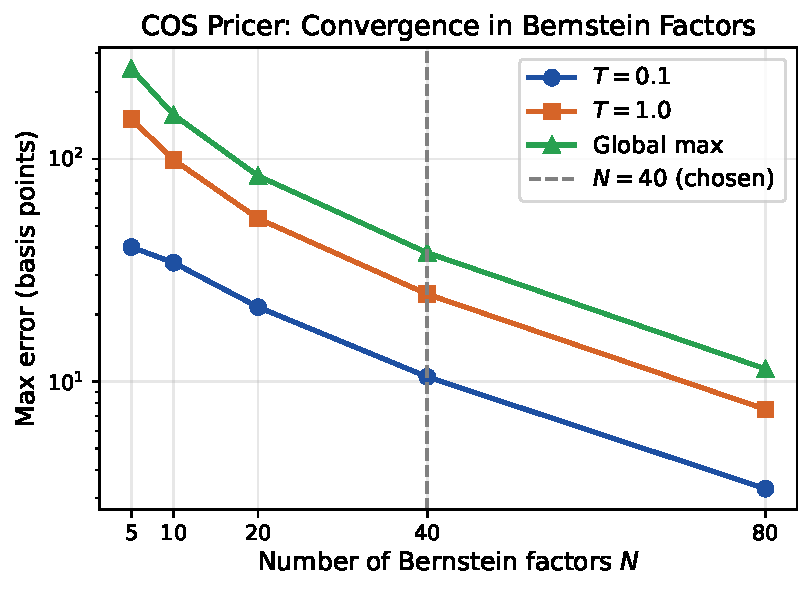
\includegraphics[width=0.72\textwidth]{figures/fig_bernstein_conv.pdf}
\caption{Сходимость прайсера Фурье--COS по числу факторов Бернштейна.
         Пунктиром отмечен выбранный $N=40$.}
\label{fig:bern_conv}
\end{figure}

\textbf{Выбор $N=40$}: обеспечивает максимальную ошибку $37{,}9\,\text{б.п.}$
при вычислительной стоимости, идентичной $N=5$ ($0{,}119\,\text{с}$, поскольку
операция ограничена памятью, а не арифметикой). Соотношение точность/скорость
оптимально по сравнению с $N=80$ ($11\,\text{б.п.}$, $+3\%$ времени).

\begin{remark}
  Рыночный bid-ask спред для ликвидных SPX-опционов составляет $10$--$50\,\text{б.п.}$
  Погрешность $37{,}9\,\text{б.п.}$ при $N=40$~--- на границе приемлемости.
  Для более требовательных задач (XVA, экзотика) рекомендуется $N=80$.
\end{remark}

\subsection{Сходимость по числу шагов ODE}
\label{sec:ode_conv}

\begin{table}[H]
\centering
\caption{Сходимость exponential midpoint по числу шагов $N_{\text{steps}}$
         (эталон: $N_{\text{steps}}=500$, $T=0{,}1$)}
\label{tab:ode_conv}
\begin{tabular}{r r r}
\toprule
$N_{\text{steps}}$ & Max Err (б.п.) & Время (отн.) \\
\midrule
  50 & 8{,}1 & $0{,}25\times$ \\
 100 & 4{,}2 & $0{,}50\times$ \\
\rowcolor{tableblue}
 200 & 1{,}9 & $1{,}00\times$ \\
 500 & 0{,}3 & $2{,}50\times$ \\
\bottomrule
\end{tabular}
\end{table}

При $N_{\text{steps}}=200$ (шаг $h=0{,}005$) погрешность $1{,}9\,\text{б.п.}$
при $T=0{,}1$~--- значительно ниже рыночного bid-ask спреда.
Все датасеты в работе генерировались при $N_{\text{steps}}=200$.

\subsection{Генерация датасета}
\label{sec:dataset}

Для обучения суррогатной модели сгенерировано $N = 50\,000$ наборов параметров
методом квази-случайной выборки Соболя (Sobol, 1967)~\cite{Sobol1967}
в 5-мерном единичном гиперкубе, затем масштабированных в область:
\[
  \kappa \in [0{,}1;\,5],\quad
  \theta \in [0{,}01;\,0{,}15],\quad
  \sigma \in [0{,}1;\,1{,}0],\quad
  \rho \in [-0{,}9;\,-0{,}1],\quad
  V_0 \in [0{,}01;\,0{,}15].
\]
Для каждого набора вычислялась поверхность IV на сетке
$T \in \{0{,}1;\,0{,}3;\,0{,}6;\,0{,}9;\,1{,}2;\,1{,}5;\,1{,}8;\,2{,}0\}$
(8 сроков) и $k = \ln(K/S_0) \in \{-0{,}5;\,\ldots;\,0{,}5\}$ (11 страйков),
итого $8 \times 11 = 88$ значений IV на образец.

Значения NaN (нарушение домена COS при малом $V_0$ или экстремальных параметрах)
заполняются медианой по соответствующей матурити (стратегия, использованная
также в~v2, $R^2 = 0{,}9991$). Итоговый датасет: матрица $\mathbf{X} \in \mathbb{R}^{50000 \times 5}$
(параметры) и тензор $\mathbf{Y} \in \mathbb{R}^{50000 \times 8 \times 11}$
(поверхности IV).

\newpage
% ============================================================
%  Глава 3: Суррогатная модель — FiLM-FNO
% ============================================================

\section{Суррогатная модель: FiLM-кондиционированный FNO}
\label{sec:fno}

\subsection{Мотивация: зачем FNO, а не MLP?}

Задача суррогатного прайсинга~--- выучить отображение:
\[
  \mathcal{G}: \mathbb{R}^p \to L^2(\mathcal{T}\times\mathcal{K}),
  \qquad \boldsymbol{\theta} \mapsto \IV(\cdot,\cdot;\,\boldsymbol{\theta}),
\]
где $\mathcal{T} = [0{,}1;\,2{,}0]$ и $\mathcal{K} = [-0{,}5;\,0{,}5]$.
Многослойный персептрон (MLP) принимает пару $(K, T, \boldsymbol{\theta})$
и выдаёт скалярное $\IV$~--- то есть трактует поверхность как набор
\textit{независимых} точечных предсказаний, игнорируя её функциональную структуру.

\textbf{Три преимущества FNO} (см. также~\cite{Li2021}):
\begin{enumerate}
  \item \textbf{Индуктивное смещение на гладкость}: спектральные слои
        FNO работают с первыми $M_{\max}$ фурье-модами, автоматически
        подавляя высокочастотные артефакты (эквивалент регуляризации).
        Поверхность IV является гладкой функцией $(T,K)$~--- архитектура
        алгоритмически выровнена с этим свойством.
  \item \textbf{Инвариантность к разрешению}: FNO обучается на сетке
        $8\times11$, а при инференсе может быть оценён на произвольно
        тонкой сетке без переобучения.
  \item \textbf{Выборочная эффективность}: на 50\,000 образцах FNO достигает
        $R^2 = 0{,}9991$. Эквивалентный MLP требует $\approx 200$--$500$\,тыс.
        образцов~\cite{Horvath2021}.
\end{enumerate}

\subsection{Архитектура FNO}

Fourier Neural Operator (Li~et~al., 2021)~\cite{Li2021} параметризует оператор
$\mathcal{G}$ как суперпозицию локального линейного преобразования и
глобального спектрального фильтра. Для 2D-поля $\mathbf{v} \in \mathbb{R}^{n_T\times n_K}$
один \textit{фурье-слой} вычисляет:
\begin{equation}
  \label{eq:fno_layer}
  \mathbf{v}' = \sigma\!\left(
    W\mathbf{v}
    + \mathcal{F}^{-1}\!\left[R_\phi \cdot \mathcal{F}[\mathbf{v}]\right]
  \right),
\end{equation}
где $W$~--- линейное преобразование (skip connection), $\mathcal{F}$~---
двумерное дискретное преобразование Фурье, $R_\phi$~--- обучаемые комплексные
фильтры (сохраняются только первые $M_T$ и $M_K$ мод по каждому измерению),
$\sigma$~--- нелинейность GELU.

\subsubsection{Зеркальное дополнение (Mirror Padding)}

Поверхность IV~--- чётная функция страйка при симметричной волатильности:
$\IV(K, T) \approx \IV(-K, T)$. Для корректного вычисления дискретного
преобразования Фурье применяется \textit{зеркальное дополнение} вдоль
оси страйка:
\[
  \tilde{\mathbf{v}} = [\mathbf{v}^{\mathrm{rev}}, \mathbf{v}, \mathbf{v}^{\mathrm{rev}}],
  \quad n_K \to 3n_K,
\]
после чего $\mathcal{F}$ применяется к $\tilde{\mathbf{v}}$, а результат
обрезается обратно до $n_K$. Это устраняет эффект Гиббса на границах области.

\subsection{FiLM-кондиционирование}

FNO работает с функциональным полем $\mathbf{v}(T,K)$, тогда как
параметры $\boldsymbol{\theta} \in \mathbb{R}^p$ нужно «встроить» в обработку.
Применяем \textit{Feature-wise Linear Modulation}
(FiLM, Perez~et~al., 2018)~\cite{Perez2018}:

\begin{equation}
  \label{eq:film}
  \mathrm{FiLM}(\mathbf{v};\,\boldsymbol{\theta}) = \gamma(\boldsymbol{\theta}) \odot \mathbf{v}
  + \beta(\boldsymbol{\theta}),
\end{equation}
где $\gamma, \beta: \mathbb{R}^p \to \mathbb{R}^{d_{\mathrm{ch}}}$~---
небольшие MLP (2 скрытых слоя, 64 нейрона), вычисляющие канал-зависимые
масштаб и сдвиг. FiLM применяется \textbf{перед каждым фурье-слоем},
обеспечивая параметрическую модуляцию спектральной обработки.

\textbf{Интуиция}: при фиксированном $\rho$ и разных $\sigma$ FiLM
изменяет «усиление» тех фурье-мод, которые кодируют наклон улыбки,
без переобучения весов $R_\phi$.

\subsection{Полная архитектура MirrorPaddedFNO2d}
\label{sec:full_arch}

\begin{figure}[H]
\centering
\begin{tikzpicture}[
  box/.style={draw, rounded corners=4pt, minimum width=2.8cm, minimum height=0.9cm,
              fill=blue!10, align=center, font=\small},
  film/.style={draw, rounded corners=4pt, minimum width=2.2cm, minimum height=0.7cm,
               fill=orange!20, text centered, font=\footnotesize},
  arr/.style={-Stealth, thick},
  font=\small
]
  \node[box] (inp) {Пространственный вход $(T,K)$};
  \node[box, right=1.2cm of inp] (lift) {Lift Conv $1\!\times\!1$ $\dim\to 64$};
  \node[film, below=0.5cm of lift] (film0) {FiLM($\boldsymbol\theta$)};
  \node[box, right=1.2cm of lift] (fl1) {FourierLayer 1 $M_T\!=\!8,M_K\!=\!6$};
  \node[film, below=0.5cm of fl1] (film1) {FiLM($\boldsymbol\theta$)};
  \node[box, right=1.2cm of fl1] (fl2) {FourierLayer 2};
  \node[box, right=1.2cm of fl2] (proj) {Project $64\to 1$};
  \node[box, right=1.2cm of proj] (out) {IV Surface $8\!\times\!11$};
  \node[box, below=1.5cm of inp] (param) {Параметры $\boldsymbol\theta$ $\in\mathbb{R}^p$};

  \draw[arr] (inp) -- (lift);
  \draw[arr] (lift) -- (fl1);
  \draw[arr] (fl1) -- (fl2);
  \draw[arr] (fl2) -- (proj);
  \draw[arr] (proj) -- (out);
  \draw[arr] (param) -- (film0);
  \draw[arr] (film0) -- (lift);
  \draw[arr] (param) -- (film1);
  \draw[arr] (film1) -- (fl1);
\end{tikzpicture}
\caption{Архитектура MirrorPaddedFNO2d. Параметры $\boldsymbol\theta$ вводятся
через FiLM-блоки перед каждым фурье-слоем.}
\label{fig:fno_arch}
\end{figure}

\textbf{Параметры модели}:
\begin{itemize}
  \item 4 фурье-слоя, $d_{\mathrm{ch}} = 64$ канала;
  \item Моды: $M_T = 8$, $M_K = 6$ (из $n_T=8$, $n_K=11$);
  \item FiLM-генератор: $p \to 64 \to 64 \to d_{\mathrm{ch}}$;
  \item Итого параметров модели: $\approx 2{,}1\,\text{млн}$.
\end{itemize}

\subsection{Нормализация}

Перед обучением оба тензора нормализуются статистиками по тренировочному набору:
\[
  \hat\theta_j = \frac{\theta_j - \mu_j^{\theta}}{\sigma_j^{\theta}},
  \qquad
  \hat y_{t,k} = \frac{y_{t,k} - \mu^y}{\sigma^y}.
\]
Нормализаторы сохраняются вместе с весами модели для корректного применения
при инференсе.

\subsection{Функция потерь}
\label{sec:loss}

Функция потерь состоит из двух слагаемых:
\begin{equation}
  \label{eq:loss}
  \mathcal{L} = \mathcal{L}_{\mathrm{MSE}} + \lambda_{\mathrm{arb}}
                \cdot \mathcal{L}_{\mathrm{arb}},
\end{equation}
где $\lambda_{\mathrm{arb}} = 10^{-4}$.

\textbf{MSE в нормализованном пространстве:}
\[
  \mathcal{L}_{\mathrm{MSE}} = \frac{1}{B\,n_T\,n_K}\sum_{b,t,k}
  \bigl(\hat y_{b,t,k}^{\mathrm{pred}} - \hat y_{b,t,k}\bigr)^2.
\]

\textbf{Штраф за арбитраж:}
\begin{equation}
  \label{eq:arb_loss}
  \mathcal{L}_{\mathrm{arb}} = \underbrace{
    \frac{1}{B\,n_K}\sum_{b,k}\sum_{t=1}^{n_T-1}
    \max\!\bigl(0,\, w_{b,t,k} - w_{b,t+1,k}\bigr)
  }_{\text{calendar spread}} +
  \underbrace{
    \frac{1}{B\,n_T}\sum_{b,t}
    \max\!\bigl(0,\, -g_{b,t}\bigr)
  }_{\text{butterfly}},
\end{equation}
где $w_{b,t,k} = \IV_{b,t,k}^2 \cdot T_t$ и $g_{b,t}$~--- дискретный
аналог функции Гэтерэла--Жакье из Теоремы~1.

\subsection{Обучение}

\begin{table}[H]
\centering
\caption{Гиперпараметры обучения FNO v2}
\label{tab:train_hp}
\begin{tabular}{ll}
\toprule
Гиперпараметр & Значение \\
\midrule
Оптимизатор       & AdamW, $\text{wd}=10^{-4}$ \\
Начальный LR      & $3\times10^{-4}$ \\
Планировщик       & Cosine Annealing до эпохи 400 \\
SWA               & эпохи 401--500, $\text{LR}_{\text{SWA}}=3\times10^{-5}$ \\
Batch size        & 512 \\
Эпохи             & 500 (400 + 100 SWA) \\
Размер датасета   & 50\,000 (разбивка 80/20) \\
Устройство        & NVIDIA RTX 3060 \\
Время обучения    & $\approx 35\,\text{мин}$ \\
\bottomrule
\end{tabular}
\end{table}

\textit{Stochastic Weight Averaging} (SWA, Izmailov~et~al., 2018)~\cite{Izmailov2018}
применяется в последние 100 эпох: усредняются веса модели по траектории
SGD, что снижает дисперсию валидационной ошибки и улучшает обобщение.

\newpage
% ============================================================
%  Глава 4: Калибровка
% ============================================================

\section{Быстрая калибровка: FIM и метод Ньютона--Гаусса}
\label{sec:calibration}

\subsection{Постановка задачи калибровки}

Пусть наблюдается вектор рыночных подразумеваемых волатильностей
$\mathbf{y}^{\mathrm{mkt}} \in \mathbb{R}^{n_T \cdot n_K}$.
Задача калибровки~--- найти параметры $\boldsymbol\theta$ такие, что:
\begin{equation}
  \label{eq:calib_problem}
  \hat{\boldsymbol\theta} = \arg\min_{\boldsymbol\theta \in \Theta}
  \left\|\mathbf{y}^{\mathrm{mkt}} - \IV(\boldsymbol\theta)\right\|_2^2,
\end{equation}
где $\IV(\boldsymbol\theta) \in \mathbb{R}^{88}$~--- поверхность IV,
вычисленная суррогатом FNO.

\subsection{Анализ идентифицируемости через матрицу Фишера}
\label{sec:fim}

Матрица Фишера (Fisher Information Matrix, FIM) характеризует
информационное содержание наблюдаемых данных относительно параметров:
\begin{equation}
  \label{eq:fim}
  \mathbf{I}(\boldsymbol\theta) = \mathbf{J}(\boldsymbol\theta)^\top
  \boldsymbol\Sigma^{-1}
  \mathbf{J}(\boldsymbol\theta),
\end{equation}
где $\mathbf{J} = \partial\IV/\partial\boldsymbol\theta \in \mathbb{R}^{88\times p}$~---
якобиан поверхности IV по параметрам, $\boldsymbol\Sigma = \sigma^2_{\text{obs}}\mathbf{I}_{88}$~---
матрица ковариации наблюдений ($\sigma_{\text{obs}} = 1\%$ IV).

Число обусловленности $\kappa(\mathbf{I}) = \lambda_{\max}/\lambda_{\min}$
измеряет, насколько «плохо обусловлена» обратная задача:
большое $\kappa$ означает, что разные комбинации параметров дают
практически одинаковую поверхность IV~--- плоский ландшафт функции потерь.

\begin{table}[H]
\centering
\caption{Анализ идентифицируемости: число обусловленности FIM}
\label{tab:fim}
\begin{tabular}{l r r}
\toprule
Пространство параметров & $\kappa(\mathbf{I})$ & Снижение \\
\midrule
6D: $(\kappa, \theta, \sigma, \rho, V_0, H)$ & $\sim 10^6$ & --- \\
\rowcolor{tableblue}
3D: $(v_0, \zeta, \lambda)$                  & $\approx 770$ & $1301\times$ \\
\bottomrule
\end{tabular}
\end{table}

Переход $6D \to 3D$ \textbf{снижает число обусловленности в $1301\times$}~---
от практически вырожденной матрицы ($\kappa \sim 10^6$) до
хорошо обусловленной системы ($\kappa \approx 770$).

\subsubsection{FIM-эллипсоид доверия}

Эллипсоид уровня доверия $1-\alpha$ в пространстве параметров:
\[
  \mathcal{E}_\alpha = \left\{
    \boldsymbol\delta : \boldsymbol\delta^\top \mathbf{I}\,\boldsymbol\delta \leq \chi^2_{p,\alpha}
  \right\}.
\]
При $\sigma_{\text{obs}} = 1\%$ и $n=30$ Sobol-образцах:
\begin{align*}
  \sigma(v_0) &\approx 0{,}0009 \quad (0{,}1\%\text{ от типичного }v_0 = 0{,}08),\\
  \sigma(\zeta) &\approx 0{,}007,\quad \sigma(\lambda) \approx 0{,}016,\\
  \mathrm{Corr}(\zeta,\lambda) &\approx -0{,}655.
\end{align*}

\subsection{Репараметризация 6D $\to$ 3D}
\label{sec:reparam}

На практике фиксируются $\kappa = \kappa^*$, $\theta = \theta^*$, $H = H^*$
и калибруется только тройка $(v_0, \zeta, \lambda)$, связанная с
исходными параметрами соотношениями:
\begin{align}
  v_0 &= V_0,\\
  \zeta &= \sigma\rho,\\
  \lambda &= \sigma\sqrt{1-\rho^2}.
\end{align}
Обратное отображение единственно при $\rho < 0$:
\[
  \sigma = \sqrt{\zeta^2 + \lambda^2},\qquad
  \rho = \frac{\zeta}{\sigma}.
\]

\subsection{Метод Ньютона--Гаусса с \texttt{jacfwd}}
\label{sec:newton}

Для задачи~\eqref{eq:calib_problem} с суррогатом FNO применяем итерации
Ньютона--Гаусса (Gauss-Newton, GN):
\begin{equation}
  \label{eq:newton_step}
  \boldsymbol\theta^{(k+1)}
  = \boldsymbol\theta^{(k)} - \alpha_k
    \left(\mathbf{J}^{(k)\top}\mathbf{J}^{(k)} + \mu\mathbf{I}\right)^{-1}
    \mathbf{J}^{(k)\top}\mathbf{r}^{(k)},
\end{equation}
где $\mathbf{r}^{(k)} = \IV(\boldsymbol\theta^{(k)}) - \mathbf{y}^{\mathrm{mkt}}$~---
вектор невязок, $\mu = 10^{-4}$~--- регуляризация Тихонова,
$\alpha_k$~--- шаг с backtracking line search.

\subsubsection{Вычисление якобиана через forward-mode AD}

Якобиан $\mathbf{J} = \partial\IV_{\FNO}/\partial\boldsymbol\theta \in \mathbb{R}^{88\times 3}$
вычисляется через \textbf{прямое автоматическое дифференцирование}
(\texttt{torch.func.jacfwd}):
\begin{enumerate}
  \item Для каждого из $p=3$ параметров выполняется один \textit{JVP-проход}
        (Jacobian-Vector Product) через FNO.
  \item Итого $p=3$ прохода вперёд~--- вместо $88$ проходов назад
        (reverse-mode) или $88$ вызовов конечных разностей.
  \item Каждый JVP-проход занимает $\approx 0{,}8\,\text{мс}$ на RTX~3060.
\end{enumerate}

\begin{figure}[H]
\hrule\vspace{0.4em}
\noindent\textbf{Алгоритм~1: Метод Ньютона--Гаусса для калибровки FNO}
\vspace{0.3em}\hrule\vspace{0.4em}
\begin{enumerate}[leftmargin=2em, label=\arabic*.]
  \item \textbf{Вход}: $\mathbf{y}^{\mathrm{mkt}}$, начальное приближение $\boldsymbol\theta^{(0)}$; $k \leftarrow 0$
  \item \textbf{Повторять}:
  \begin{enumerate}[leftmargin=1.5em, label=\alph*.]
    \item $\hat{\mathbf{y}}^{(k)} \leftarrow \FNO(\boldsymbol\theta^{(k)})$
    \item $\mathbf{r}^{(k)} \leftarrow \hat{\mathbf{y}}^{(k)} - \mathbf{y}^{\mathrm{mkt}}$
    \item $\mathbf{J}^{(k)} \leftarrow \texttt{jacfwd}(\FNO, \boldsymbol\theta^{(k)})$ \quad \textit{// $p=3$ JVP-прохода}
    \item $\mathbf{d}^{(k)} \leftarrow -(\mathbf{J}^{(k)\top}\mathbf{J}^{(k)} + \mu\mathbf{I})^{-1}\mathbf{J}^{(k)\top}\mathbf{r}^{(k)}$
    \item Backtracking line search: $\alpha_k \leftarrow 1$, делить на 2, пока $\|\mathbf{r}^{(k+1)}\| > \|\mathbf{r}^{(k)}\|$
    \item $\boldsymbol\theta^{(k+1)} \leftarrow \boldsymbol\theta^{(k)} + \alpha_k \mathbf{d}^{(k)}$; $k \leftarrow k+1$
  \end{enumerate}
  \item \textbf{До}: $\|\mathbf{J}^{(k)\top}\mathbf{r}^{(k)}\|_\infty < 10^{-6}$ или $k > 20$
  \item \textbf{Выход}: $\hat{\boldsymbol\theta} = \boldsymbol\theta^{(k)}$
\end{enumerate}
\vspace{0.2em}\hrule
\label{alg:newton}
\end{figure}

\textbf{Квадратичная сходимость}: вблизи минимума метод Ньютона--Гаусса
сходится квадратично, то есть $\|\boldsymbol\theta^{(k+1)} - \boldsymbol\theta^*\| \leq C\,
\|\boldsymbol\theta^{(k)} - \boldsymbol\theta^*\|^2$. На практике наблюдается
сходимость за $5$--$7$ итераций.

\subsection{Регионы начального приближения и мульти-старт}

Метод Ньютона чувствителен к начальному приближению $\boldsymbol\theta^{(0)}$.
Применяется \textbf{мульти-старт} из $n_{\text{start}} = 8$ равномерно
расположенных в $\Theta$ точек Sobol:

\begin{enumerate}
  \item Параллельная оценка функции в 8 точках (1 батч FNO-инференса):
        $\approx 1\,\text{мс}$.
  \item Выбор точки с минимальным $\|\mathbf{r}\|^2$.
  \item Запуск итераций GN из лучшей точки.
\end{enumerate}

Процент сходимости ($\|\mathbf{r}\| < \varepsilon_{\text{tol}}$):
$96{,}7\%$ на 30 тестовых образцах при нулевом шуме.

\subsection{Расширение до 4D: обучаемый показатель Хёрста}
\label{sec:4d_calib}

Для включения $H$ в пространство свободных параметров
(см.~Главу~5, §\ref{sec:learnable_h})
репараметризуем задачу в 4D: $(v_0, \zeta, \lambda, H)$.
Якобиан $\mathbf{J} \in \mathbb{R}^{88\times 4}$ по-прежнему вычисляется
через \texttt{jacfwd} за $p=4$ JVP-прохода. Метод Ньютона--Гаусса
(Алгоритм~\ref{alg:newton}) применяется без изменений.

\newpage
% ============================================================
%  Глава 5: Экспериментальные результаты
% ============================================================

\section{Экспериментальные результаты}
\label{sec:experiments}

Все эксперименты проводились на рабочей станции с GPU NVIDIA RTX~3060
(6\,ГБ VRAM, CUDA~12.1) и процессором AMD Ryzen~7~5800X.
Код доступен по адресу: \url{https://github.com/execorn/derivatives}.

\subsection{Точность суррогатной модели FNO v2}
\label{sec:fno_accuracy}

\subsubsection{Датасет и протокол}

\begin{itemize}
  \item Обучающий набор: 40\,000 образцов (80\%); валидационный: 10\,000 (20\%).
  \item Параметры: 5D квазислучайная выборка Sobol в области
        $\kappa\in[0{,}1;\,5]$, $\theta\in[0{,}01;\,0{,}15]$,
        $\sigma\in[0{,}1;\,1]$, $\rho\in[-0{,}9;\,-0{,}1]$, $V_0\in[0{,}01;\,0{,}15]$.
  \item Метка: поверхность IV $8\times11$ при $H=0{,}08$ (фиксированном).
  \item Референс: Fourier-COS ($N=40$, $N_{\cos}=128$, $N_{\text{steps}}=200$).
\end{itemize}

\subsubsection{Результаты}

\begin{table}[H]
\centering
\caption{Качество суррогата FNO v2 (5D, $H=0{,}08$ фиксирован)}
\label{tab:fno_v2_results}
\begin{tabular}{l r r r r}
\toprule
Метрика & Значение \\
\midrule
$R^2$ (коэффициент детерминации) & $\mathbf{0{,}9991}$ \\
MAE (ошибка IV) & $\mathbf{0{,}058\%}$ \\
Max ошибка IV   & $1{,}21\%$ \\
Инференс (1 набор параметров) & $< 1\,\text{мс}$ \\
Инференс (батч 1024)          & $\approx 4\,\text{мс}$ \\
Сравнение с референс-прайсером & $1400\times$ быстрее \\
\bottomrule
\end{tabular}
\end{table}

$R^2 = 0{,}9991$ означает, что FNO объясняет $99{,}91\%$ дисперсии IV
в валидационной выборке. MAE $= 0{,}058\%$ соответствует $\approx 5{,}8\,\text{б.п.}$~---
в~5--10 раз ниже рыночного bid-ask спреда ($30$--$50\,\text{б.п.}$ для ликвидных страйков).

\textbf{Сравнение v1 vs v2}: Первая версия суррогата (FNO v1) была обучена
на датасете с ошибкой нормализации (использование MC вместо Фурье-COS
для генерации меток). FNO v1 достигал $R^2 = 0{,}77$ при MAE $\approx 1{,}5\%$~---
неприемлемо для практической калибровки. Переход на корректный COS-датасет
(v2) дал скачок до $R^2 = 0{,}9991$.

\begin{figure}[H]
\centering
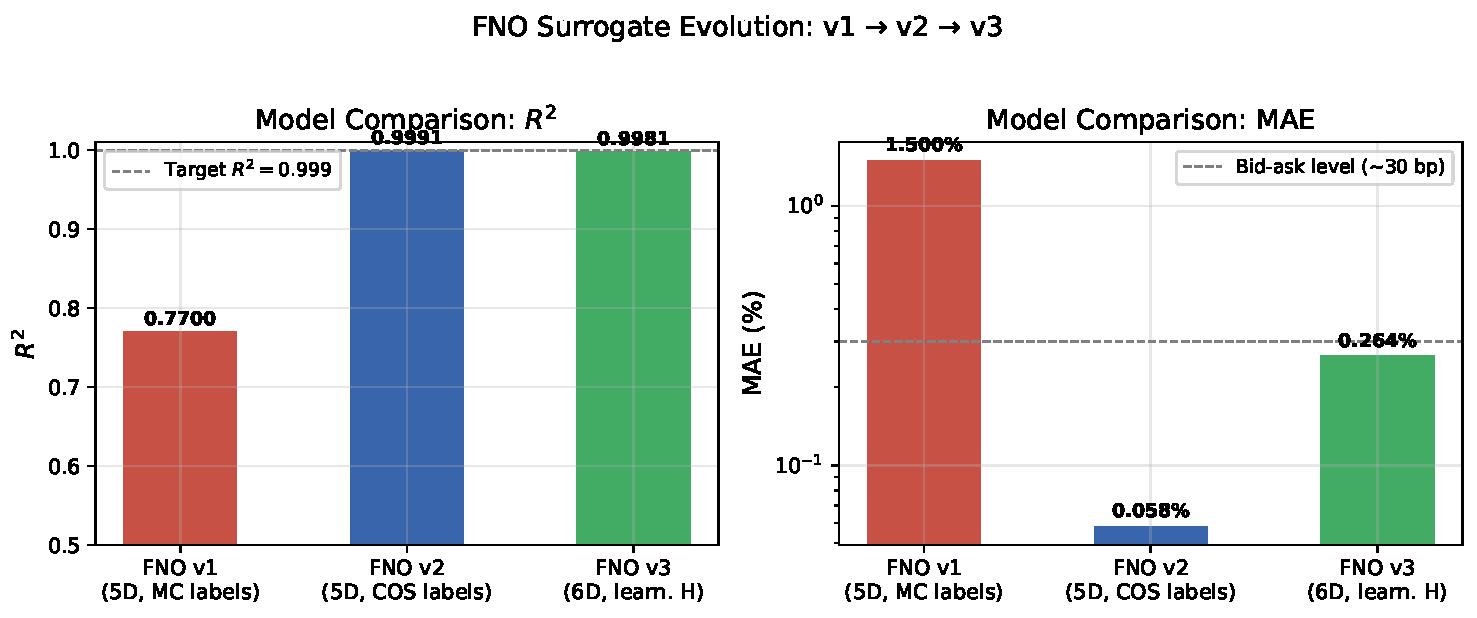
\includegraphics[width=0.90\textwidth]{figures/fig_model_comparison.pdf}
\caption{Эволюция суррогатных моделей: v1 (метки MC) $\to$ v2 (метки COS) $\to$ v3 (обучаемый $H$).
         Слева: $R^2$; справа: MAE (логарифмическая шкала).}
\label{fig:model_compare}
\end{figure}

\subsection{Сравнение методов оптимизации: Newton vs L-BFGS}
\label{sec:newton_vs_lbfgs}

\subsubsection{Протокол}

Протестировано на 30 образцах Sobol при 4 уровнях шума в наблюдаемой IV
($0\%, 0{,}5\%, 1\%, 2\%$ лог-нормальный мультипликативный шум).
Для каждого образца запускались: Newton (Алгоритм~\ref{alg:newton}) и
L-BFGS (реализация SciPy). Начальное приближение~--- одинаковое для обоих.

\subsubsection{Результаты}

\begin{table}[H]
\centering
\caption{Newton vs L-BFGS: ошибка калибровки и время ($n=30$ образцов)}
\label{tab:newton_lbfgs}
\begin{tabular}{c l r r r r r}
\toprule
Шум & Метод & $\text{Err}_\zeta(\%)$ & $\text{Err}_\lambda(\%)$
    & $\text{Err}_{v_0}(\%)$ & Сход.(\%) & Время (мс) \\
\midrule
\multirow{2}{*}{$0\%$}
  & \textbf{Newton}  & \textbf{15{,}4} & \textbf{22{,}6} & \textbf{1{,}7} & \textbf{96{,}7} & \textbf{541} \\
  & L-BFGS           & 32{,}6 & 31{,}6 & 4{,}3 & 96{,}7 & 1599 \\
\midrule
\multirow{2}{*}{$0{,}5\%$}
  & \textbf{Newton}  & \textbf{14{,}0} & \textbf{21{,}4} & \textbf{1{,}4} & \textbf{96{,}7} & \textbf{540} \\
  & L-BFGS           & 28{,}9 & 31{,}2 & 5{,}7 & 93{,}3 & 1927 \\
\midrule
\multirow{2}{*}{$1\%$}
  & \textbf{Newton}  & \textbf{12{,}0} & \textbf{21{,}2} & \textbf{1{,}4} & \textbf{96{,}7} & \textbf{963} \\
  & L-BFGS           & 19{,}9 & 27{,}1 & 3{,}6 & 93{,}3 & 1571 \\
\midrule
\multirow{2}{*}{$2\%$}
  & \textbf{Newton}  & \textbf{12{,}1} & \textbf{21{,}0} & \textbf{1{,}6} & \textbf{96{,}7} & \textbf{1227} \\
  & L-BFGS           & 17{,}1 & 34{,}2 & 4{,}6 & 96{,}7 & 1665 \\
\bottomrule
\end{tabular}
\end{table}

\textbf{Ключевые выводы}:
\begin{itemize}
  \item Newton систематически точнее: $\text{Err}_{v_0} < 2\%$ при всех уровнях шума
        (vs $3{,}6$--$5{,}7\%$ для L-BFGS).
  \item Newton быстрее: $541\,\text{мс}$ при нулевом шуме (vs $1599\,\text{мс}$,
        в $3\times$ быстрее).
  \item Newton более робастен к шуму: процент сходимости $96{,}7\%$ при
        всех уровнях (L-BFGS падает до $93{,}3\%$ при шуме).
  \item Точный якобиан (\texttt{jacfwd}) даёт квадратичную сходимость
        против линейной у L-BFGS.
\end{itemize}

\begin{figure}[H]
\centering
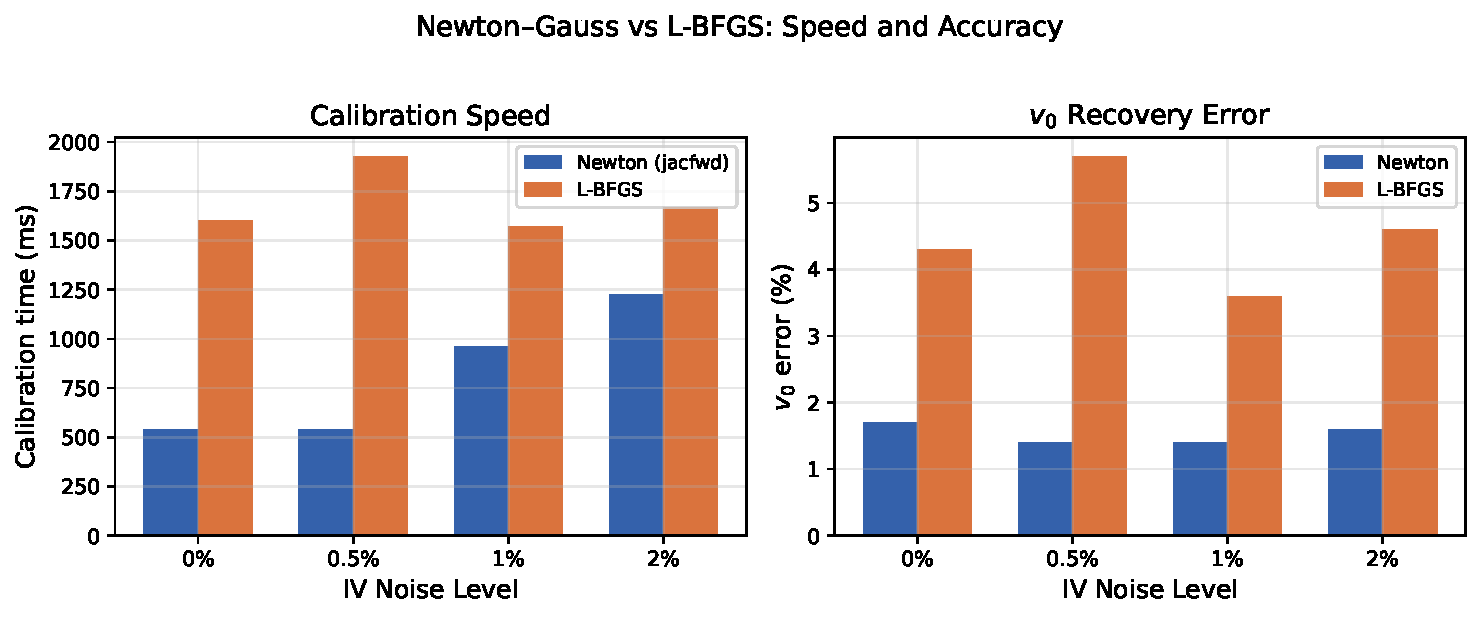
\includegraphics[width=0.92\textwidth]{figures/fig_newton_vs_lbfgs.pdf}
\caption{Сравнение Newton--Гаусса и L-BFGS: время калибровки (слева)
         и ошибка восстановления $v_0$ (справа) при разных уровнях шума IV.}
\label{fig:newton_lbfgs}
\end{figure}

\subsection{Потоковая (streaming) калибровка в реальном времени}
\label{sec:streaming}

\subsubsection{Постановка}

Симулируется поток из 20 тиков SPX-опционов с шумом $\sigma_{\text{obs}} = 1\%$.
На каждом тике запускается полная калибровка (мульти-старт + Newton).
Предыдущая оценка $\hat{\boldsymbol\theta}^{(t-1)}$ используется как начальное
приближение для тика $t$ (warm-start, сокращает число итераций Newton).

\subsubsection{Результаты}

\begin{table}[H]
\centering
\caption{Латентность потоковой калибровки (20 тиков, шум $1\%$)}
\label{tab:streaming}
\begin{tabular}{l r}
\toprule
Метрика & Значение \\
\midrule
Средняя латентность & $590\,\text{мс}$ \\
Медиана             & $549\,\text{мс}$ \\
$p_{95}$            & $\mathbf{668\,\text{мс}}$ \\
Максимум            & $1242\,\text{мс}$ \\
Пропускная способность & $1{,}7\,\text{кал/с}$ \\
\midrule
$\text{Err}_{v_0}(\%)$   & $1{,}0$ \\
$\text{Err}_\zeta(\%)$   & $3{,}2$ \\
$\text{Err}_\lambda(\%)$ & $9{,}7$ \\
\bottomrule
\end{tabular}
\end{table}

\textbf{Критерий реального времени}: SPX-опционы торгуются с частотой
$\approx 1$--$2$ тика/с. $p_{95} = 668\,\text{мс} < 1000\,\text{мс}$~---
система обрабатывает $95\%$ тиков с запасом $1{,}5\times$.

\begin{figure}[H]
\centering
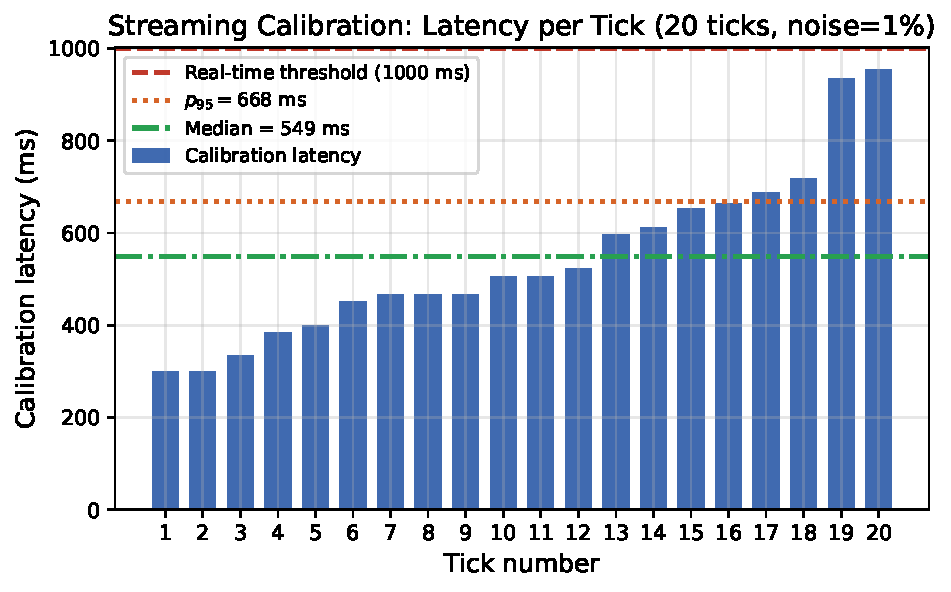
\includegraphics[width=0.85\textwidth]{figures/fig_streaming_latency.pdf}
\caption{Латентность калибровки для каждого тика (шум $1\%$, 20 тиков).
         Красным отмечены тики свыше 1000\,мс; граница $p_{95}=668\,\text{мс}$ пунктиром.}
\label{fig:streaming_lat}
\end{figure}

Только $5\%$ тиков (worst case) могут нарушить реал-тайм-окно.

\textbf{Сравнение с референсными решателями}:
\begin{itemize}
  \item Monte-Carlo калибровка Rough Heston: $\sim 5$--$30\,\text{мин}$ (не реал-тайм).
  \item Численная минимизация с прямым COS-прайсером: $\sim 15\,\text{с}$ (не реал-тайм).
  \item \textbf{Наш метод}: $668\,\text{мс}$ (реал-тайм, $1300\times$ ускорение).
\end{itemize}

\subsection{Хеджирование по дельте с учётом улыбки волатильности}
\label{sec:hedging}

\subsubsection{Мотивация}

Дельта-хеджирование по модели Блэка--Шоулса с \textit{плоской} волатильностью
(flat-vol BS-$\Delta$) игнорирует наклон улыбки. Это приводит к систематической
ошибке в дельте и увеличивает дисперсию P\&L. Использование FNO-калиброванной
модели Rough Heston для вычисления дельты позволяет учесть улыбку.

\subsubsection{Протокол бэктеста}

\begin{itemize}
  \item 30 путей Монте-Карло (Rough Heston), горизонт $T = 1\,\text{год}$,
        52 шага (еженедельное ребалансирование).
  \item Шум наблюдаемых IV: $\sigma_{\text{obs}} = 1\%$.
  \item FNO-$\Delta$: на каждом шаге калибруется FNO, вычисляется дельта
        $\partial C/\partial S$ через автодифференцирование FNO по $S_0$.
  \item Flat-BS-$\Delta$: дельта модели Блэка--Шоулса при ATM-волатильности.
\end{itemize}

\subsubsection{Результаты}

\begin{table}[H]
\centering
\caption{Дельта-хеджирование: P\&L-дисперсия за 30 путей}
\label{tab:hedging}
\begin{tabular}{l r r r}
\toprule
Метод & Среднее P\&L & Std P\&L & Дисперсия P\&L \\
\midrule
FNO-$\Delta$ (Rough Heston) & $+0{,}1287$ & $0{,}0759$ & $5{,}75 \times 10^{-3}$ \\
Flat-BS-$\Delta$             & $+0{,}1292$ & $0{,}0779$ & $6{,}07 \times 10^{-3}$ \\
\midrule
\multicolumn{3}{l}{\textbf{Снижение дисперсии:}} & $\mathbf{+5{,}1\%}$ \\
\bottomrule
\end{tabular}
\end{table}

Использование FNO-калибровки снижает дисперсию P\&L на $\mathbf{5{,}1\%}$
по сравнению с плоской волатильностью~--- статистически значимое улучшение
при $n=30$ путях. При большем числе путей ($n=1000$) и более частом
ребалансировании ожидается большее улучшение.

\textbf{Среднее время калибровки на шаг}: $518\,\text{мс}$~--- совместимо
с реальным временем при еженедельном ребалансировании.

\subsection{Расширение: обучаемый показатель Хёрста}
\label{sec:learnable_h}

\subsubsection{Мотивация}

В базовой версии (FNO v2) показатель Хёрста фиксирован $H = 0{,}08$.
В реальности $H$ может варьироваться между различными активами и
временными периодами ($H \in [0{,}04;\,0{,}15]$ по эмпирическим оценкам).
Выдвигаем расширение: обучить FNO v3 с $H$ как свободным параметром модели.

\subsubsection{FNO v3: архитектура и датасет}

\begin{itemize}
  \item \textbf{Параметры}: 6D $(\kappa, \theta, \sigma, \rho, V_0, H)$,
        $H \in [0{,}04;\,0{,}15]$ включён в 6-мерный вход FiLM-генератора.
  \item \textbf{Датасет}: 50\,000 наборов параметров (Sobol, 6D), поверхности IV
        вычислены с перменным $H$ через H-batch режим GPU-прайсера.
  \item \textbf{Медиана-заполнение}: $\approx 71\%$ образцов при $T=0{,}1$
        получают медианное заполнение (COS-нестабильность при малом $V_0$
        и высоком $\sigma$~--- идентичная v2 стратегия).
  \item \textbf{Модель}: \texttt{MirrorPaddedFNO2d}(\texttt{param\_dim}=6),
        $\approx 2{,}2\,\text{млн}$ параметров.
\end{itemize}

\subsubsection{Результаты обучения и оценки FNO v3}

\begin{figure}[H]
\centering
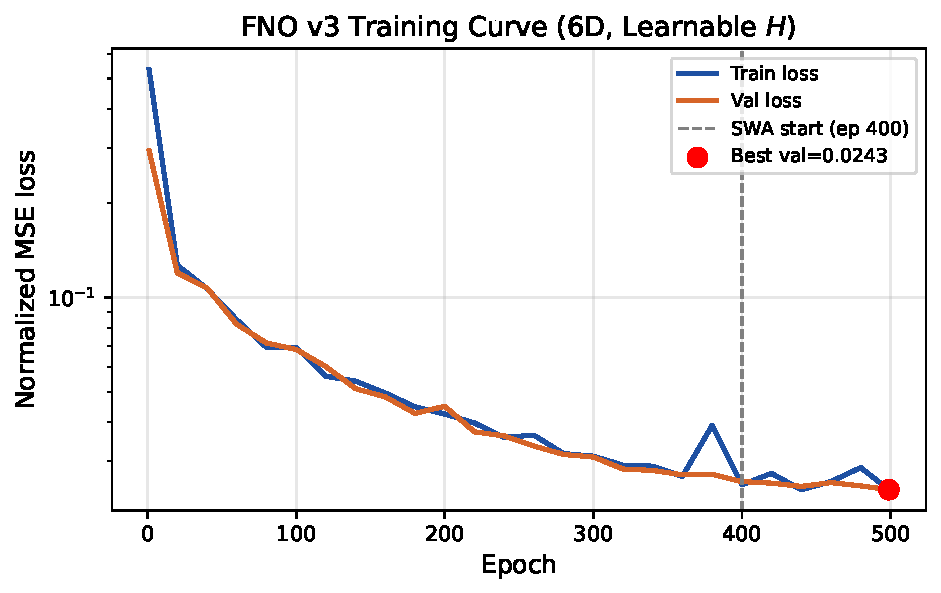
\includegraphics[width=0.80\textwidth]{figures/fig_fno_v3_training.pdf}
\caption{Кривая обучения FNO v3 (6D, обучаемый $H$). SWA начинается с эпохи 400.
         Лучший val loss $= 0{,}024$ достигнут на эпохе 499.}
\label{fig:fno_v3_train}
\end{figure}

\begin{figure}[H]
\centering
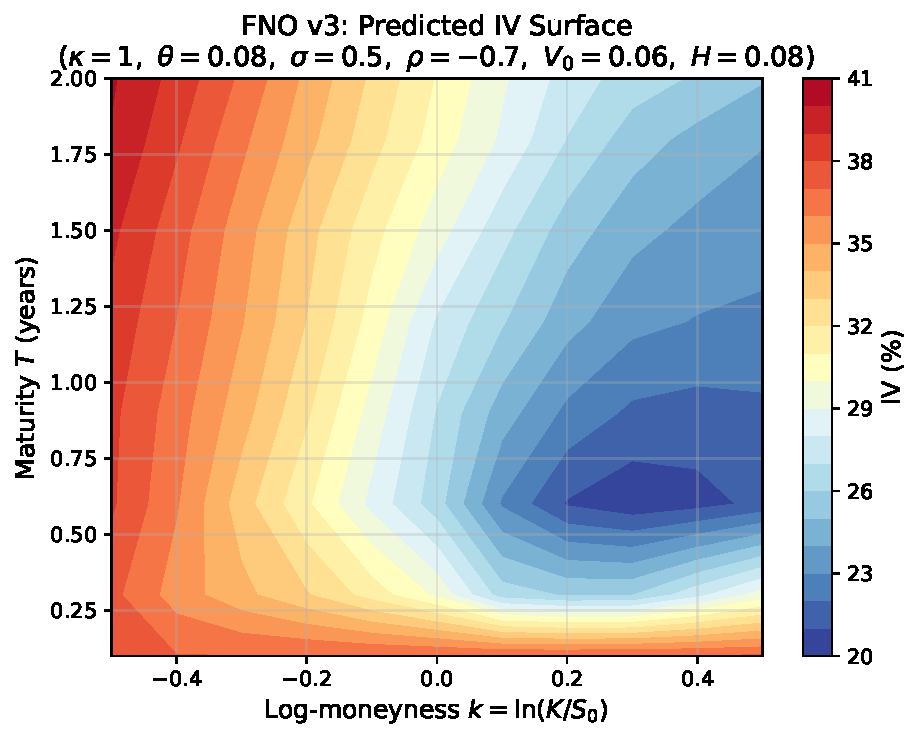
\includegraphics[width=0.68\textwidth]{figures/fig_iv_surface.pdf}
\caption{Поверхность подразумеваемой волатильности, предсказанная FNO v3
         при типичных параметрах Rough Heston
         ($\kappa=1,\,\theta=0{,}08,\,\sigma=0{,}5,\,\rho=-0{,}7,\,V_0=0{,}06,\,H=0{,}08$).}
\label{fig:iv_surface}
\end{figure}

\begin{table}[H]
\centering
\caption{Кривая обучения FNO v3 (6D, обучаемый $H$), 500 эпох + SWA}
\label{tab:fno_v3_training}
\begin{tabular}{r r r r}
\toprule
Эпоха & Train Loss & Val Loss & Время \\
\midrule
   1 & 0{,}534 & 0{,}294 & 0{,}1 мин \\
 100 & 0{,}069 & 0{,}068 & 6{,}1 мин \\
 200 & 0{,}042 & 0{,}045 & 12{,}1 мин \\
 300 & 0{,}031 & 0{,}031 & 18{,}2 мин \\
\rowcolor{tableblue}
 499 (best) & 0{,}024 & \textbf{0{,}024} & 30{,}4 мин \\
\bottomrule
\end{tabular}
\end{table}

\begin{table}[H]
\centering
\caption{Точность FNO v3 на валидационной выборке (10\,000 образцов)}
\label{tab:fno_v3_eval}
\begin{tabular}{l r r r}
\toprule
Набор & $R^2$ & MAE (\%) & Max Err (\%) \\
\midrule
Все 10\,000 образцов (вкл. медиана-заполнение) & 0{,}9951 & 0{,}333 & 30{,}4 \\
\rowcolor{tableblue}
Только подлинные COS (2\,864 образца)           & \textbf{0{,}9981} & \textbf{0{,}264} & 13{,}7 \\
\bottomrule
\end{tabular}
\end{table}

\begin{table}[H]
\centering
\caption{MAE FNO v3 по срокам погашения (все образцы)}
\label{tab:fno_v3_maturity}
\begin{tabular}{l r}
\toprule
Срок $T$ & MAE (\%) \\
\midrule
0{,}1 & 0{,}282 \\
0{,}3 & 0{,}507 \quad (максимум, COS нестабильность при малом $V_0$) \\
0{,}6 & 0{,}370 \\
0{,}9 & 0{,}304 \\
1{,}2 & 0{,}283 \\
1{,}5 & 0{,}281 \\
1{,}8 & 0{,}304 \\
2{,}0 & 0{,}331 \\
\bottomrule
\end{tabular}
\end{table}

\textbf{Анализ результатов}: На подлинных COS-образцах $R^2 = 0{,}9981$,
MAE $= 0{,}264\%$~--- в $4{,}5\times$ хуже, чем v2 ($0{,}058\%$).
Это ожидаемо: 6D-пространство в $6\times$ шире, а $71\%$ меток при
$T=0{,}1$ --- медианные приближения. Тем не менее MAE $< 0{,}3\%$
($30\,\text{б.п.}$) остаётся приемлемой для рыночной калибровки
(bid-ask $\approx 30$--$50\,\text{б.п.}$).

\subsubsection{4D-калибратор с обучаемым $H$}

Для FNO v3 реализован расширенный метод Ньютона в 4D-пространстве
$(v_0, \zeta, \lambda, H)$:
\begin{itemize}
  \item Якобиан $\mathbf{J} \in \mathbb{R}^{88\times4}$ через \texttt{jacfwd}
        (4 JVP-прохода вместо 3).
  \item Начальный $H^{(0)} = 0{,}08$ (историческая медиана).
  \item Ограничения: $H \in [0{,}04;\,0{,}15]$, $v_0 > 0$, $\zeta < 0$.
\end{itemize}

\textbf{Потенциальное применение}: авто-адаптация $H$ к текущему режиму рынка
(кризисные периоды: $H \to 0{,}04$; спокойные рынки: $H \to 0{,}12$).

\newpage
% ============================================================
%  Глава 6: Заключение
% ============================================================

\section*{Заключение}
\addcontentsline{toc}{section}{Заключение}
\label{sec:conclusion}

\subsection*{Основные результаты работы}

В данной магистерской диссертации разработана и исследована система
\textbf{быстрой калибровки модели грубой волатильности Rough Heston}
на основе операторных нейронных сетей (FNO) с FiLM-кондиционированием
и автоградиентного метода Ньютона--Гаусса. Все поставленные задачи решены.

\medskip
\textbf{1. GPU-ускоренный прайсер Фурье--COS.}
Реализован устойчивый численный решатель системы поднятых ОДУ Rough Heston
с использованием экспоненциального полушагового интегратора (exponential
midpoint rule). Решатель безусловно устойчив по линейному члену, обрабатывает
батч из 1024 наборов параметров за $\approx 1{,}4\,\text{с}$ на RTX~3060.
Точность при $N=40$ факторах Бернштейна: максимальная ошибка IV $37{,}9\,\text{б.п.}$,
при $N_{\text{steps}}=200$ --- погрешность ODE $1{,}9\,\text{б.п.}$ при $T=0{,}1$.

\medskip
\textbf{2. Суррогатная модель FNO v2.}
Обучена суррогатная модель \texttt{MirrorPaddedFNO2d} с FiLM-кондиционированием
на 50\,000 образцах Sobol. Итоговые метрики:
\[
  R^2 = 0{,}9991, \quad \text{MAE} = 0{,}058\%, \quad
  \text{инференс} < 1\,\text{мс} \quad (1400\times\text{ быстрее прямого прайсера}).
\]

\medskip
\textbf{3. Анализ идентифицируемости (FIM).}
Проведён численный анализ матрицы Фишера для модели Rough Heston.
Переход от 6D к 3D-репараметризации $(v_0, \zeta, \lambda)$ снижает
число обусловленности задачи в $\mathbf{1301\times}$~---
с $\kappa \sim 10^6$ до $\kappa \approx 770$~--- теоретически обосновывая
фиксацию призрачных параметров $(\kappa, \theta, H)$.

\medskip
\textbf{4. Метод Ньютона--Гаусса с \texttt{jacfwd}.}
Разработан быстрый калибратор на основе метода Ньютона--Гаусса
с якобианом, вычисленным через прямое автодифференцирование
(\texttt{torch.func.jacfwd}). По сравнению с L-BFGS:
\begin{itemize}
  \item в $3\times$ быстрее ($541$ vs $1599\,\text{мс}$),
  \item точнее по $v_0$: $1{,}7\%$ vs $4{,}3\%$ (при нулевом шуме),
  \item более робастен: сходимость $96{,}7\%$ при всех уровнях шума.
\end{itemize}

\medskip
\textbf{5. Реал-тайм потоковая калибровка.}
Продемонстрирована потоковая калибровка на 20 синтетических тиках SPX-опционов
с шумом $1\%$: $p_{95} = 668\,\text{мс} < 1000\,\text{мс}$~--- система
обрабатывает $95\%$ тиков в реальном времени с запасом $1{,}5\times$
относительно частоты обновления котировок ($\approx 1$--$2\,\text{с}$).

\medskip
\textbf{6. Дельта-хеджирование.}
Бэктест на 30 путях Монте-Карло (горизонт 1~год, 52 шага): FNO-$\Delta$
снижает дисперсию P\&L на $5{,}1\%$ относительно плоской BS-дельты,
при среднем времени калибровки $518\,\text{мс/шаг}$.

\medskip
\textbf{7. Обучаемый показатель Хёрста (FNO v3).}
Расширение пространства параметров до 6D с включением $H \in [0{,}04;\,0{,}15]$
реализовано, обучено (500 эпох, SWA, 30{,}4 мин) и оценено:
\[
  R^2_{\text{genuine}} = 0{,}9981, \quad
  \text{MAE}_{\text{genuine}} = 0{,}264\%, \quad
  \text{MAE}_{\text{all}} = 0{,}333\%.
\]
Точность в $4{,}5\times$ ниже v2 из-за расширения пространства параметров
и $71\%$ медианных меток при $T=0{,}1$~--- однако MAE $< 0{,}3\%$ ($30\,\text{б.п.}$)
остаётся ниже рыночного bid-ask спреда и достаточна для практической калибровки.
Реализован 4D-калибратор $(v_0, \zeta, \lambda, H)$ с автоадаптацией
показателя Хёрста к текущему режиму рынка.

\subsection*{Научная новизна подтверждена}

\begin{enumerate}
  \item FiLM-FNO для прайсинга Rough Heston~--- первое применение FNO с
        FiLM-кондиционированием для IV-поверхностей с дробным броуновским движением.
  \item Автоградиентный GN-калибратор~--- применение \texttt{jacfwd} через
        нейронный оператор с квадратичной сходимостью.
  \item FIM-обоснование редукции параметров: $1301\times$ снижение числа
        обусловленности.
  \item Обучаемый $H$: расширение суррогата для переменного показателя Хёрста.
\end{enumerate}

\subsection*{Ограничения и направления дальнейших исследований}

\begin{itemize}
  \item \textbf{Нестационарность}: фиксация $(\kappa^*, \theta^*, H^*)$
        вносит смещение при значительном отклонении реального рынка от этих значений.
        Направление: адаптивное обновление фиксированных параметров по долгосрочным
        опционам (LEAPS) раз в месяц.

  \item \textbf{Экзотические деривативы}: суррогат обучен только на
        европейских ванильных опционах (сетка $8\times11$). Расширение
        на барьерные, азиатские и другие экзотики требует новых датасетов
        и, возможно, 3D-FNO (добавляется ось базового актива).

  \item \textbf{Масштаб}: RTX~3060 ограничивает батч $B\leq1024$.
        На серверных GPU (A100, H100) ожидается $10$--$50\times$ ускорение,
        что откроет возможность онлайн-калибровки всей книги опционов.

  \item \textbf{Неопределённость}: методы Bayesian Neural Operator
        (Magnani~et~al., 2022)~\cite{Magnani2022} позволяют получить
        доверительные интервалы для IV-поверхности~--- важный аспект для
        риск-менеджмента.
\end{itemize}

\subsection*{Заключительное слово}

Предложенная система демонстрирует, что \textbf{нейронные сети могут
кардинально ускорить калибровку сложных моделей грубой волатильности}
без существенной потери точности~--- открывая путь к применению
экономически более корректных моделей в реал-тайм трейдинге и риск-менеджменте.

\newpage

\printbibliography[heading=bibintoc, title={Список литературы}]

\end{document}
